% Standalone staged subsection; not inserted into the existing manuscript.
\subsection{Training-step proxy}
\label{sec:phase4-training-proxy}

To examine whether the sparse-index accumulation effects observed in isolated
measurements persist in a broader backpropagation-style setting, we introduced a
small synthetic training-step proxy. The proxy combines indexed lookup, grouped
mean pooling, a scalar linear prediction head, mean-squared error, and backward
propagation. The three variants use identical inputs, pooling, head, and loss.
The \texttt{embedding\_\allowbreak backward\_\allowbreak proxy} variant uses native dense Embedding
backward, whereas \texttt{index\_\allowbreak add\_\allowbreak proxy} and
\texttt{scatter\_\allowbreak add\_\allowbreak proxy} use custom autograd lookup nodes that allocate a
dense zero gradient and accumulate row gradients with the corresponding PyTorch
API.

Two timing scopes were recorded. The \texttt{proxy\_\allowbreak step} scope measures the
complete synthetic step: lookup, pooling, prediction, loss, and gradients for the
table, head, and bias. The \texttt{accumulation\_\allowbreak region} scope separately replays
backward through a retained lookup graph with fixed upstream gradients. This
second scope is diagnostic only: it includes autograd dispatch, dense gradient
allocation and zeroing, and accumulation, but it is not an exact decomposition of
the proxy step and must not be subtracted from total-step latency.

Each environment was evaluated with five seeds and 24 configurations per seed,
giving 120 seed--configuration observations per environment. The grid varied the
number of rows, number of references, embedding dimension, and index
distribution. All included runs completed successfully, and all configurations
and variants passed the recorded validation checks. As in the preceding
experiments, a variant is counted as a winner only when the runner-up median is
strictly more than 5\% slower; otherwise the observation is classified as a
practical tie.

Table~\ref{tab:phase4-winner-counts} and
Figure~\ref{fig:phase4-winner-counts} summarize the results. On the GTX1650Ti stack, \texttt{index\_\allowbreak add} dominated both scopes, winning 83 of 120
proxy-step observations and 98 of 120 accumulation-region observations. Native
Embedding won 10 observations in each scope, while the remaining cases were
classified as practical ties. On the T4 stack, practical ties dominated: 95 of
120 proxy-step observations and 78 of 120 accumulation-region observations. Among
the resolved T4 cases, the proxy step favored \texttt{scatter\_\allowbreak add} in 25
observations, while the accumulation-region diagnostic favored
\texttt{scatter\_\allowbreak add} in 39 observations and \texttt{index\_\allowbreak add} in three.

\begin{table*}[t]
\centering\fontsize{9}{11}\selectfont
\caption{Phase~4 winners under the strictly greater than 5\% practical-margin rule. Each environment contributes 120 seed--configuration observations. Region replay denotes the separate accumulation diagnostic scope.}
\label{tab:phase4-winner-counts}
\setlength{\tabcolsep}{3pt}
\renewcommand{\arraystretch}{1.12}
\begin{tabular*}{\textwidth}{@{\extracolsep{\fill}}llrrrrr@{}}
\toprule
Environment & Scope & \texttt{index\_add} & \texttt{scatter\_add} & Embedding & Tie & Total \\
\midrule
GTX1650Ti & Proxy step & 83 & 0 & 10 & 27 & 120 \\
GTX1650Ti & Region replay & 98 & 0 & 10 & 12 & 120 \\
T4 & Proxy step & 0 & 25 & 0 & 95 & 120 \\
T4 & Region replay & 3 & 39 & 0 & 78 & 120 \\
\bottomrule
\end{tabular*}
\end{table*}
% \begin{table}[tbp]
\centering\fontsize{9}{11}\selectfont
\caption{Descriptive Phase~4 outcomes by environment. The contrast is not attributed to GPU hardware alone because the software and host environments also differ.}
\label{tab:phase4-environment-comparison}
\setlength{\tabcolsep}{3pt}
\begin{tabularx}{\linewidth}{lXXX}
\toprule
Environment & Proxy-step outcome & Region-replay outcome & Interpretation \\
\midrule
GTX1650Ti & \texttt{index\_add}: 83/120 & \texttt{index\_add}: 98/120 & The local stack most often favors the custom \texttt{index\_add} path. \\
T4 & Tie: 95/120 & Tie: 78/120 & Most observations are unresolved; resolved cases mainly favor \texttt{scatter\_add}. \\
\bottomrule
\end{tabularx}
\end{table}

\begin{figure*}[t]
\centering
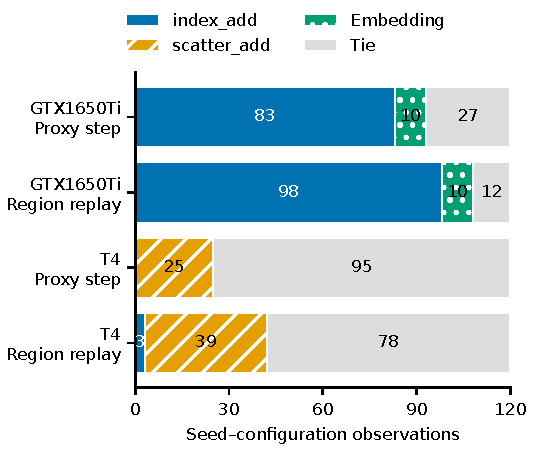
\includegraphics[width=0.60\linewidth]{figures/phase4_winner_counts_by_environment.pdf}
\caption{Phase~4 practical-margin winner counts across five seeds and 24
configurations per environment. Region replay denotes the separate accumulation
diagnostic scope. Ties are retained explicitly.}
\label{fig:phase4-winner-counts}
\end{figure*}

The proxy results reinforce the central conclusion that sparse-index accumulation
performance is conditional rather than universal. In the GTX1650Ti stack, the custom \texttt{index\_\allowbreak add} backward path was most often favored.
In the T4 stack, most observations were unresolved by the 5\% practical
margin rule, and the resolved cases mainly favored \texttt{scatter\_\allowbreak add}. This
contrast should not be interpreted as isolated GPU causality, because the two
environments also differ in PyTorch version, CUDA version, operating system, and
host settings. Instead, the result shows that rankings obtained from isolated
sparse-index accumulation measurements should not be transferred mechanically to
a training-step-like context without measurement.

This proxy remains deliberately limited. It does not measure convergence,
optimizer state, data loading, distributed training, or production-scale model
throughput. The manual variants use custom autograd lookup nodes, so the
comparison is at the API/path level and includes dispatch and graph overhead
rather than pure kernel speed. The \texttt{accumulation\_\allowbreak region} scope is a
diagnostic replay, not a decomposition of the proxy step.